\section{自己開示を促す楽曲推薦システム}
本節では，システムの基本設計について述べる．

\begin{comment}
\subsection{要件}
選曲を通じた自己開示を促すには，システムに以下のような要件が必要である．

\subsection*{要件1. 個人の楽曲に対する自己開示レベルの定量化}
システムが自己開示を促進するうえでは，定量化する必要がある．

\subsection*{要件2. 段階的な自己開示の制御}
要件1で定量化した自己開示レベルについて，レベルの低い楽曲から高い楽曲へと段階的に開示を促す必要がある．

\subsection*{要件3. ユーザーの選曲過程や，受容度の変化を記録する}
要件2の段階的にシステムが提示した曲と，ユーザーの選択した曲の変化，すなわち要件1の自己開示レベルの変化を時系列的に記録できるシステムである必要がある．

\vskip\baselineskip

これらの要件を～．
\end{comment}

\subsection{3軸の分類基準}

本項では，\ref{3軸}項で整理した自己開示の3軸についての取得方法，定量化方法を検討する．「思い入れ」と「歌うことの自信」は，個人の主観であり，客観的指標として取得することが不可能である．そのため，主観指標として曲に対して表\ref{tab:evaluation_criteria}に示すように4段階で被験者に評価をさせることとした．

\begin{table}[htbp]
\centering
\caption{楽曲の評価基準}
\label{tab:evaluation_criteria}
\begin{tabular}{|c|c|c|}
\hline
評価値 & 思い入れ & 歌うことの自信 \\
\hline
1 & ほとんど思い入れがない & ほとんど自信がない \\
2 & あまり思い入れがない & あまり自信がない \\
3 & やや思い入れがある & やや自信がある \\
4 & とても強い思い入れがある & とても自信がある \\
\hline
\end{tabular}
\end{table}

楽曲の人気度については，個々人間で知っている/知らない曲を完全に網羅することは難しく，人により曲の認知度は違って感じられるため，主観指標を使うことは難しい．そのため，Spotify Web API\cite{SpotifyWebAPI}から取得できるpopularityという客観的な数値（0-100）を使用する．これら3つの指標に基づき，各楽曲の自己開示レベルを定量的に評価する．

次項では，各軸の数値から自己開示レベルを決定する方法について述べる．


\subsection{自己開示レベルの区分}

\ref{3軸}項での3軸に基づき，カラオケにおける自己開示を4つのレベルに分類する．既存の研究ではこのような自己開示の段階を定義した手法は存在しない．そのため，今回は各軸の値を活かすため，2分法を用いて表\ref{tab:自己開示レベルの分類}のように分類を行うこととした．

思い入れと歌うことの自信は，表\ref{tab:evaluation_criteria}の4段階評価から，1-2の値を低い，3-4を高いとする．人気度については，Spotify APIから取得した1-100の値を，50を閾値として高低の2値に変換する．なお，思い入れが低く（1-2），歌唱への自信も低く（1-2），人気度も低い（50未満）楽曲については，開示者の感情表現も乏しく，被開示者からの受容も得られにくいことから適切に機能しないと判断し，分類から除外する．
% この分類では，思い入れを主軸とし，歌唱への自信と人気度を補助的な要素として扱う．

\begin{table}[H]
\centering
\caption{自己開示レベルの分類}
\begin{tabular}{|c|c|c|c|}
\hline
自己開示レベル & 思い入れ & 歌える自信 &  人気度  \\
\hline
1 & ない & ある & 高い \\
\hline
1 & ない & ない & 高い \\
\hline
2 & ない & ある & 低い \\
\hline
2 & ある & ある & 高い \\
\hline
3 & ある & ない & 高い \\
\hline
3 & ある & ある & 低い \\
\hline
4 & ある & ない & 低い \\
\hline
- & ない & ない & 低い \\
\hline
\end{tabular}
\label{tab:自己開示レベルの分類}
\end{table}


\subsection{実装}
提案したシステム設計に基づき，Webアプリケーションとして実装を行った．本項では，使用した開発環境，事前準備と本実験のデータフローについて説明する．

\vskip.5\baselineskip

システムの実装には，表\ref{tab:libraries}に示すライブラリとフレームワークを使用した．アプリケーションのベースとしてNode.js 20.17.0を採用し，フロントエンド・バックエンドの統合フレームワークとしてNext.js\cite{NextJS}を使用した．
データベースにはSupabase\cite{Supabase}を採用し，データベース管理を行った．また，楽曲情報の取得にはSpotify Web APIを利用し，next-authとiron-sessionを用いてAPI認証を実装した．
本アプリケーションは実験被験者が実際に使用することを想定し，安定した運用環境としてVercel\cite{Vercel}を使用した．


\begin{table}[H]
\caption{システム作成に使用したライブラリ・バージョン}
\label{tab:libraries}
\begin{center}
\begin{tabular}{|l|c||l|c|} \hline
\multicolumn{4}{|c|}{Node.js 20.17.0} \\ \hline
ライブラリ & バージョン & ライブラリ & バージョン \\ \hline
@mui/material & 6.3.1 & @supabase/supabase-js & 2.47.10 \\
axios & 1.7.9 & iron-session & 8.0.4 \\
next & 15.1.3 & next-auth & 4.24.11 \\
react & 19.0.0 & tailwindcss & 3.4.1 \\
typescript & 5.7.2 & & \\ \hline
\end{tabular}
\end{center}
\end{table}

\ref{実験手順}項の実験手順を満たすような事前準備のデータフローを図\ref{fig:事前準備のデータフロー}に，本実験の音楽共有セッションでのデータフローを図\ref{fig:音楽共有セッションのデータフロー}に示す．

\begin{figure}[H]
    \centering
    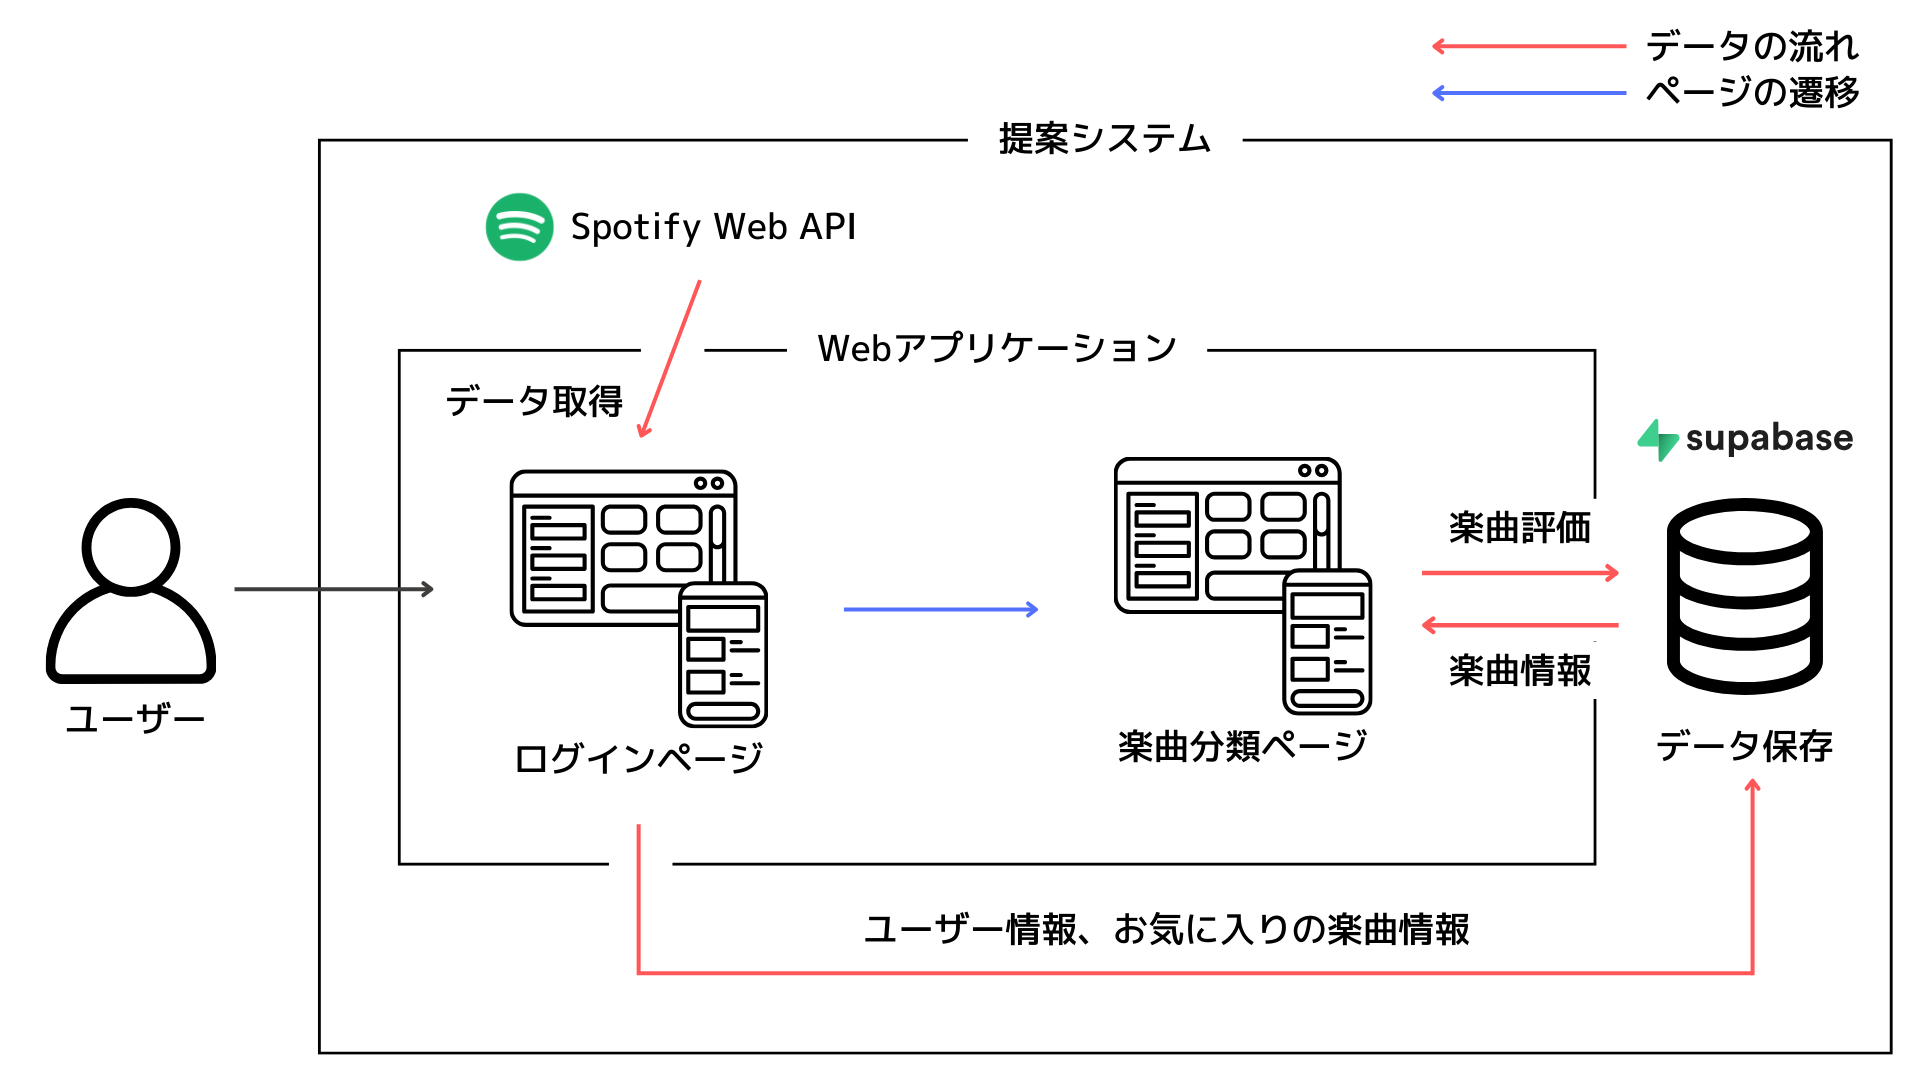
\includegraphics[width=1\linewidth]{image/data-flow-chart1.png}
    \caption{事前準備のデータフロー}
    \label{fig:事前準備のデータフロー}
\end{figure}

\begin{figure}[H]
    \centering
    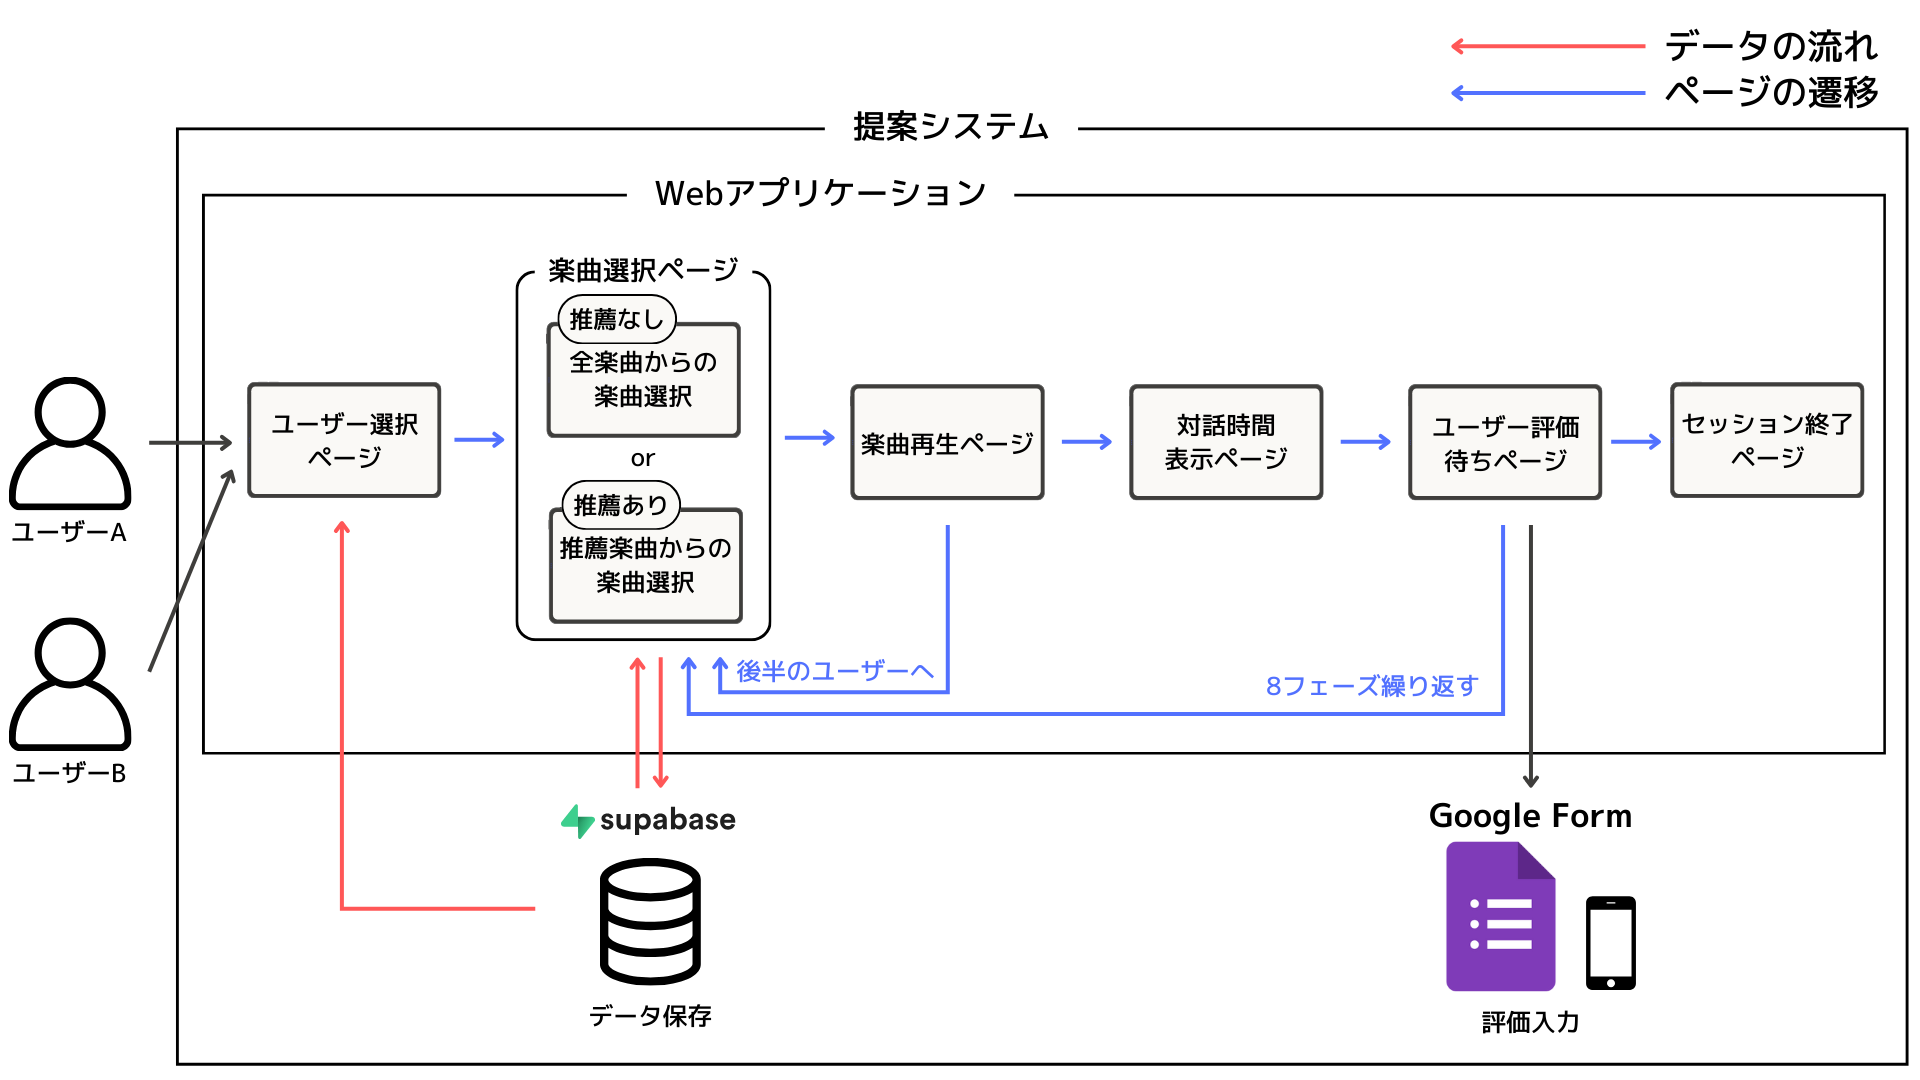
\includegraphics[width=1\linewidth]{image/data-flow-chart2.png}
    \caption{音楽共有セッションのデータフロー}
    \label{fig:音楽共有セッションのデータフロー}
\end{figure}
